\documentclass[a4paper,twocolumn,11pt,accepted=2024-02-08]{quantumarticle}
\pdfoutput=1
\usepackage[T1]{fontenc}
\usepackage{amsmath,amsfonts,amssymb,amsthm,bbm,bm, braket}
\usepackage[numbers]{natbib}
\usepackage{wasysym}
\usepackage{comment}
\usepackage{scalerel}
\usepackage{enumerate}
\usepackage{amssymb}
\usepackage{graphicx}
\usepackage{mathtools}
\usepackage{ifthen}
\usepackage{tensor}
\usepackage{tikz}
\usepackage{tikz-network}
%\usetikzlibrary{shapes.geometric}%added
\usetikzlibrary{patterns,decorations.pathreplacing}

\usepackage{color}
\usepackage{longtable}%Added!
\usepackage[normalem]{ulem} % either use this (simple) 

\theoremstyle{break}        
\newtheorem{Prop}{Property} %\newtheorem{Prop}{Property}[section]
\newtheorem{Lemma}{Lemma}
%\newtheorem{Lemma}{Lemma}[section]
\newtheorem{Proposition}{Proposition}
%\newtheorem{Proposition}{Proposition}[section]
\usepackage{color}
\definecolor{myred}{RGB}{232,102,102}
\definecolor{myblue}{RGB}{187,187,255}
\definecolor{myorange0}{RGB}{252,226,5}
\definecolor{myorange0c}{RGB}{255,255,255}
\definecolor{myorange}{RGB}{255,165,0}
\definecolor{mygrey}{RGB}{105,105,105}
\definecolor{OliveGreen}{RGB}{85,107,47}
\definecolor{NavyBlue}{RGB}{0,0,128}
%\definecolor{myY}{RGB}{220,255,203}
\definecolor{mygreen}{RGB}{34,139,34}
\definecolor{myY}{RGB}{220,255,203}
\definecolor{myYO}{RGB}{255, 220, 151}

\definecolor{mygreenc}{RGB}{150,50,50}

\usepackage{tensor}
\newcommand{\be}{\begin{equation}}
\newcommand{\ee}{\end{equation}}
\newcommand{\ba}{\begin{aligned}}
\newcommand{\ea}{\end{aligned}}
\newcommand{\bw}{\begin{widetext}}
\newcommand{\ew}{\end{widetext}}
\newcommand{\1}{\mathbbm{1}}
\newtheorem{theorem}{Theorem}
\theoremstyle{plain}
\newtheorem{property}{Property}
\theoremstyle{plain}
\newtheorem{lemma}{Lemma}
\theoremstyle{plain}
\newtheorem{observation}{Observation}
\usepackage[colorlinks,bookmarks=false,citecolor=NavyBlue,linkcolor=OliveGreen,urlcolor=blue]{hyperref}




\DeclareMathOperator{\arccosh}{arcCosh}
\newcommand{\du}{{\rm du}}

\renewcommand{\qedsymbol}{$\blacksquare$}

\newcommand{\Wgatedagger}[2]{
\draw[very thick] (#1-0.5, #2 +0.5) -- (#1+0.5,#2-0.5);
\draw[very thick] (#1-0.5,#2-0.5) -- (#1+0.5,#2+0.5);
\draw[ thick, fill=mygreenc, rounded corners=2pt] (#1-0.25,#2+0.25) rectangle (#1+0.25,#2-0.25);
\draw[thick] (#1,#2+0.15) -- (#1+0.15,#2+0.15) -- (#1+0.15,#2);
%\Text[x=0,y=-0.075]{\x \y}
}
\newcommand{\Wgatered}[2]{
\draw[very thick] (#1-0.5, #2 +0.5) -- (#1+0.5,#2-0.5);
\draw[very thick] (#1-0.5,#2-0.5) -- (#1+0.5,#2+0.5);
\draw[ thick, fill=myred, rounded corners=2pt] (#1-0.25,#2+0.25) rectangle (#1+0.25,#2-0.25);
\draw[thick] (#1,#2+0.15) -- (#1+0.15,#2+0.15) -- (#1+0.15,#2);
%\Text[x=0,y=-0.075]{\x \y}
}
\newcommand{\Wgateblue}[2]{
\draw[very thick] (#1-0.5, #2 +0.5) -- (#1+0.5,#2-0.5);
\draw[very thick] (#1-0.5,#2-0.5) -- (#1+0.5,#2+0.5);
\draw[ thick, fill=myblue, rounded corners=2pt] (#1-0.25,#2+0.25) rectangle (#1+0.25,#2-0.25);
\draw[thick] (#1,#2+0.15) -- (#1+0.15,#2+0.15) -- (#1+0.15,#2);
%\Text[x=0,y=-0.075]{\x \y}
}

\newcommand{\WgateblueT}[2]{
\draw[very thick] (#1-0.5, #2 +0.5) -- (#1+0.5,#2-0.5);
\draw[very thick] (#1-0.5,#2-0.5) -- (#1+0.5,#2+0.5);
\draw[ thick, fill=myblue, rounded corners=2pt] (#1-0.25,#2+0.25) rectangle (#1+0.25,#2-0.25);
\draw[thick] (#1,#2-0.15) -- (#1+0.15,#2-0.15) -- (#1+0.15,#2);
%\Text[x=0,y=-0.075]{\x \y}
}
\newcommand{\Wgategreen}[2]{
\draw[very thick] (#1-0.5, #2 +0.5) -- (#1+0.5,#2-0.5);
\draw[very thick] (#1-0.5,#2-0.5) -- (#1+0.5,#2+0.5);
\draw[ thick, fill=mygreen, rounded corners=2pt] (#1-0.25,#2+0.25) rectangle (#1+0.25,#2-0.25);
\draw[thick] (#1,#2+0.15) -- (#1+0.15,#2+0.15) -- (#1+0.15,#2);
%\Text[x=0,y=-0.075]{\x \y}
}
\newcommand{\MYcircle}[2]{
\draw[thick, fill=white] (#1,#2) circle (0.1cm); }
\newcommand{\MYsquare}[2]{
%\node[regular polygon,
%    draw= thick,
%    regular polygon sides = 4,
 %    fill =white,
 %    minimum size = .2cm
 %    ] (p) at (#1,#2) {}; 
 \coordinate (Origin) at (#1,#2);
\filldraw [thick, fill=white, even odd rule] ($(Origin)+(-.1cm,-.1cm)$) coordinate (Square) -- ++(0.0cm,0.2cm) -- ++(0.2cm,0.0cm) -- ++(0.0cm,-0.2cm) -- cycle;
 }
\newcommand{\MYtriangle}[2]{
 \coordinate (Origin) at (#1,#2);
\filldraw [thick, fill=white, even odd rule] ($(Origin)+(-.0cm,{0.666*cos(60)*0.3cm})$) coordinate (Triangle) -- ++(0.15cm,-{cos(60)*0.3cm}) -- ++(-0.3cm,0.0cm) -- ++(0.15cm,{cos(60)*0.3cm}) -- cycle;
}
\newcommand{\MYcircleB}[2]{
\draw[thick, fill=black] (#1,#2) circle (0.1cm); }

\newcommand{\rhoO}[2]{
\draw[very thick] (-.5+#1,0.5+#2) -- (#1,0+#2);
\draw[very thick] (#1,0+#2) -- (.5+#1,0.5+#2);
\draw[very thick] (-.5+#1,#2) -- (.5+#1,#2);
\draw[ thick, fill=mygreen, rounded corners=2pt] (-0.35+#1,0.2-0.25+#2) rectangle (0.35+#1,0.2+0.2+#2);
\draw[very thick] (0.1+#1,0.15+.18+#2)-- (.15+0.1+#1,0.15+.18+#2) -- (.15+0.1+#1,0+.18+#2);
}

\newcommand{\Wgategrey}[2]{
\draw[very thick] (#1-0.5, #2 +0.5) -- (#1+0.5,#2-0.5);
\draw[very thick] (#1-0.5,#2-0.5) -- (#1+0.5,#2+0.5);
\draw[ thick, fill=mygrey, rounded corners=2pt] (#1-0.25,#2+0.25) rectangle (#1+0.25,#2-0.25);
\draw[thick] (#1,#2+0.15) -- (#1+0.15,#2+0.15) -- (#1+0.15,#2);
%\Text[x=0,y=-0.075]{\x \y}
}
\newcommand{\mcirc}{\mathbin{\scalerel*{\fullmoon}{G}}}
\newcommand{\msquare}{\mathord{\scalerel*{\Box}{G}}}
\newcommand{\mcircf}{\mathbin{\scalerel*{\newmoon}{G}}}
\newcommand{\mtriangle}{\mathord{\scalerel*{\triangle}{G}}}
\newcommand{\MYsquareB}[2]{

\draw[ thick, fill=black, rounded corners=2pt] (#1-0.25,#2+0.25) rectangle (#1+0.25,#2-0.25);
\draw[thick, color=white] (#1,#2+0.15) -- (#1+0.15,#2+0.15) -- (#1+0.15,#2);
%\Text[x=0,y=-0.075]{\x \y}
}

\newcommand{\tr}{\text{tr} \, }
\newcommand{\Tr}{\text{Tr} \, }
%Tiles
\newcommand{\lineW}{.8mm}
\newcommand{\sroot}{1.41421356237}

%\input{HeadIncludes.txt}
\def\scale{0.3}

\newcommand{\gs}[1]{{\color{red}[#1]}}
\newcommand{\pk}[1]{{\color{blue}[#1]}}
\newcommand{\zw}[1]{{\color{orange}#1}}
\definecolor{skyblue}{RGB}{135, 206, 235}
%Set up the metadata
\hypersetup{
 pdftitle={Hierarchical generalization of dual unitarity},
 pdfsubject={Many-body systems},
 pdfauthor={Xie-Hang Yu, Xie-Hang Yu, and Pavel Kos},
 pdfkeywords={exact solutions, quantum circuits, quantum many-body systems}
}
\begin{document}
\begin{equation*}
    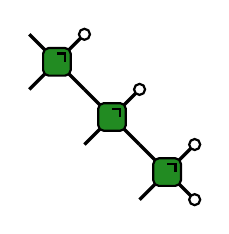
\begin{tikzpicture}[baseline=(current  bounding  box.center), scale=0.7]
    \Wgategreen{-1.5}{0.5}
    \Wgategreen{-0.5}{-0.5}
    \Wgategreen{-2.5}{1.5}
    \MYcircle{-1}{1}
    \MYcircle{0}{0}
    \MYcircle{0}{-1}
    \MYcircle{-2}{2}
    \end{tikzpicture}
    =
    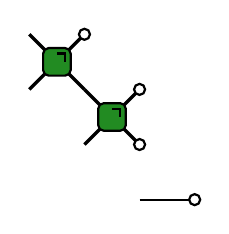
\begin{tikzpicture}[baseline=(current  bounding  box.center), scale=0.7]
    \Wgategreen{-1.5}{0.5}
    \Wgategreen{-2.5}{1.5}
    \draw[thick] (-1,-1)--(0,-1);
    \MYcircle{0}{-1}
    \MYcircle{-1}{0}
    \MYcircle{-1}{1}
    \MYcircle{-2}{2}
    \end{tikzpicture}
    .\label{eq:3rdHierarchydefinition}
\end{equation*}
\begin{equation*}
    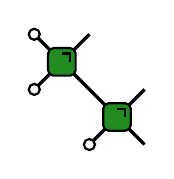
\begin{tikzpicture}[baseline=(current  bounding  box.center), scale=0.7]
        \Wgategreen{-0.5}{0.5}
        \Wgategreen{0.5}{-0.5}
        \MYcircle{-1}{1}
        \MYcircle{-1}{0}
        \MYcircle{0}{-1}
        \end{tikzpicture}
        =
        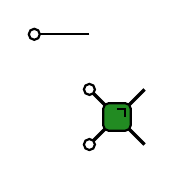
\begin{tikzpicture}[baseline=(current  bounding  box.center), scale=0.7]
        \Wgategreen{0.5}{-0.5}
        \draw[thick] (0,1)--(-1,1);
        \MYcircle{-1}{1}
        \MYcircle{0}{0}
        \MYcircle{0}{-1}
    \end{tikzpicture}
\end{equation*}
\begin{equation*}
    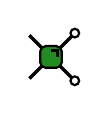
\begin{tikzpicture}[baseline=(current  bounding  box.center), scale=0.55]
        \Wgategreen{0}{0}
        \MYcircle{0.55}{0.55}
        \MYcircle{0.55}{-0.55}
        \end{tikzpicture}
        =
        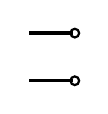
\begin{tikzpicture}[baseline=(current  bounding  box.center), scale=0.55]
        \MYcircle{0.55}{0.55}
        \MYcircle{0.55}{-0.55}
        \draw[very thick] (-0.5,0.55) -- (0.5,0.55);
        \draw[very thick] (-0.5,-0.55) -- (0.5,-0.55);
    \end{tikzpicture}
\end{equation*}
\begin{equation*}
    w=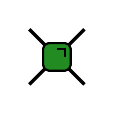
\begin{tikzpicture}[baseline=(current  bounding  box.center), scale=0.7]
    \Wgategreen{0}{0}
    \end{tikzpicture}
    =
    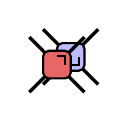
\begin{tikzpicture}[baseline=(current  bounding  box.center), scale=0.7]
    \WgateblueT{0.15}{0.07}
    \Wgatered{-0.1}{-0.07}
    \end{tikzpicture}
\end{equation*}
\begin{equation*}
    
\begin{tikzpicture}[baseline=(current  bounding  box.center), scale=0.7]
    \MYcircle{0.25}{0.25}
    \draw[very thick] (-0.25,-0.25)--(0.20,0.20);
    \end{tikzpicture}
    =\frac{1}{\sqrt{D}}
    
\begin{tikzpicture}[baseline=(current  bounding  box.center), scale=0.7]
    \draw[very thick] (-0.25,-0.25)--(0.25,0.25)--(0.05,0.45)--(-0.45,-0.05);
    \end{tikzpicture}
\end{equation*}
\end{document}
